\documentclass[letterpaper, 11pt, twocolumn]{article}
\usepackage{graphicx}
\usepackage{amsmath}
\usepackage{float}
\usepackage{geometry}
\geometry{letterpaper, margin=20mm, nohead}
\linespread{0.9}


\graphicspath{{./pics/}}
\begin{document}

\title{\vspace{-10mm} 6.013 Final Project Report}
\author{Andres Erbsen, Justin Graves, Dimitris Koutentakis}
\date{\today}
\maketitle
\vspace{5mm}
% \tableofcontents
% \clearpage
\section{Abstract}
From 6.013 we learned that transmission lines can resonate at certain
frequencies and create standing waves based on the geometry and reflection
coefficients at the boundaries of the lines. We used this concept to design,
build, and characterize two band-pass filters (achieving 20dB stop-band
attenuation) based on TEM resonators and two band-stop filters that produce a
smith chart short at the stop frequency (achieving 35dB attenuation).

\section {Introduction}
Filters are very important components in a multitude of applications that are
essential to our day-to-day lives. They are vital in communication receivers and
transmitters in order select channel reception, block interference from various
sources as well as avoid transmission in unwanted frequencies that can have
technical as well as legal implications.  There is a variety of ways to build
electronic filters, the most simple of which are lumped component RLC 
circuits. However, the above-mentioned often use frequencies in multiple MHz and
GHz, and building lumped-element filters is increasingly difficult at higher
frequencies.  If we wanted to build lumped
element circuit filters for our 2.4 GHz radar
frequency, we would need an LC product of $10^{-10}\text{s}^2$. Given an
inter-trace capacitance of 1pF, we would need inductors as small as 10nH.
A simple wire (or PCB trace) would have inductance higher than that.

In order to solve this problem we designed, developed and debugged a series of
band stop and band pass filters made by microstrips. Microstrips allow us to
design and build some highly accurate filters with straightforward tools and
manufacturing processes.

\section{Approach}
In order to design our filters, we had to apply some of the basic knowledge we acquired in the lectures towards the end of the semester. More specifically, we had to apply knowledge regarding transmission line resonators as well as smith charts and stubs.
\\
By calculating the dimensions for our given substrate and target frequencies we were able to build the filters desired. The filters that we ended up building are:
\begin{itemize}
    \item A short-short half wave resonator built with the dimensions of the original substrate board,
    \item A short-short half wave resonator for $f=2.4 GHz$,
    \item A single stub band-stop resonator, and
    \item A multi-band-stop filter with sharp passband edges
\end{itemize}
\subsection{Half wave resonator band-pass filter}
For the first short-short half-wave resonator, we used the dimensions of the original board given. More specifically, we used the width of the board, $D=7.7cm$ and $\delta$ very small (\(\delta<0.8cm\) in order to maximize our $Q$. Given the width of our board and the material with $\epsilon_r=2.33$, we calculated a wavelength of \(\lambda_0=2\cdot D \cdot\sqrt(\epsilon_r)=23.5cm\), corresponding to a resonant frequency of $f=\frac{c}{\lambda_0}=1.277GHz$.
% \begin{align*}
%     D=7.7cm &\Rightarrow \frac{\lambda_n}{D}=7.7cm \\
%     \lambda_0=7.7cm\cdot2\cdot\sqrt{2.33}&\Rightarrow \lambda_0=23.5cm \\
%     f=\frac{3\cdot10^{8}}{23.5\cdot10^{-2}} &\Rightarrow f=1.277 GHz
% \end{align*}

% \begin{figure}[H]
%     \centering
%     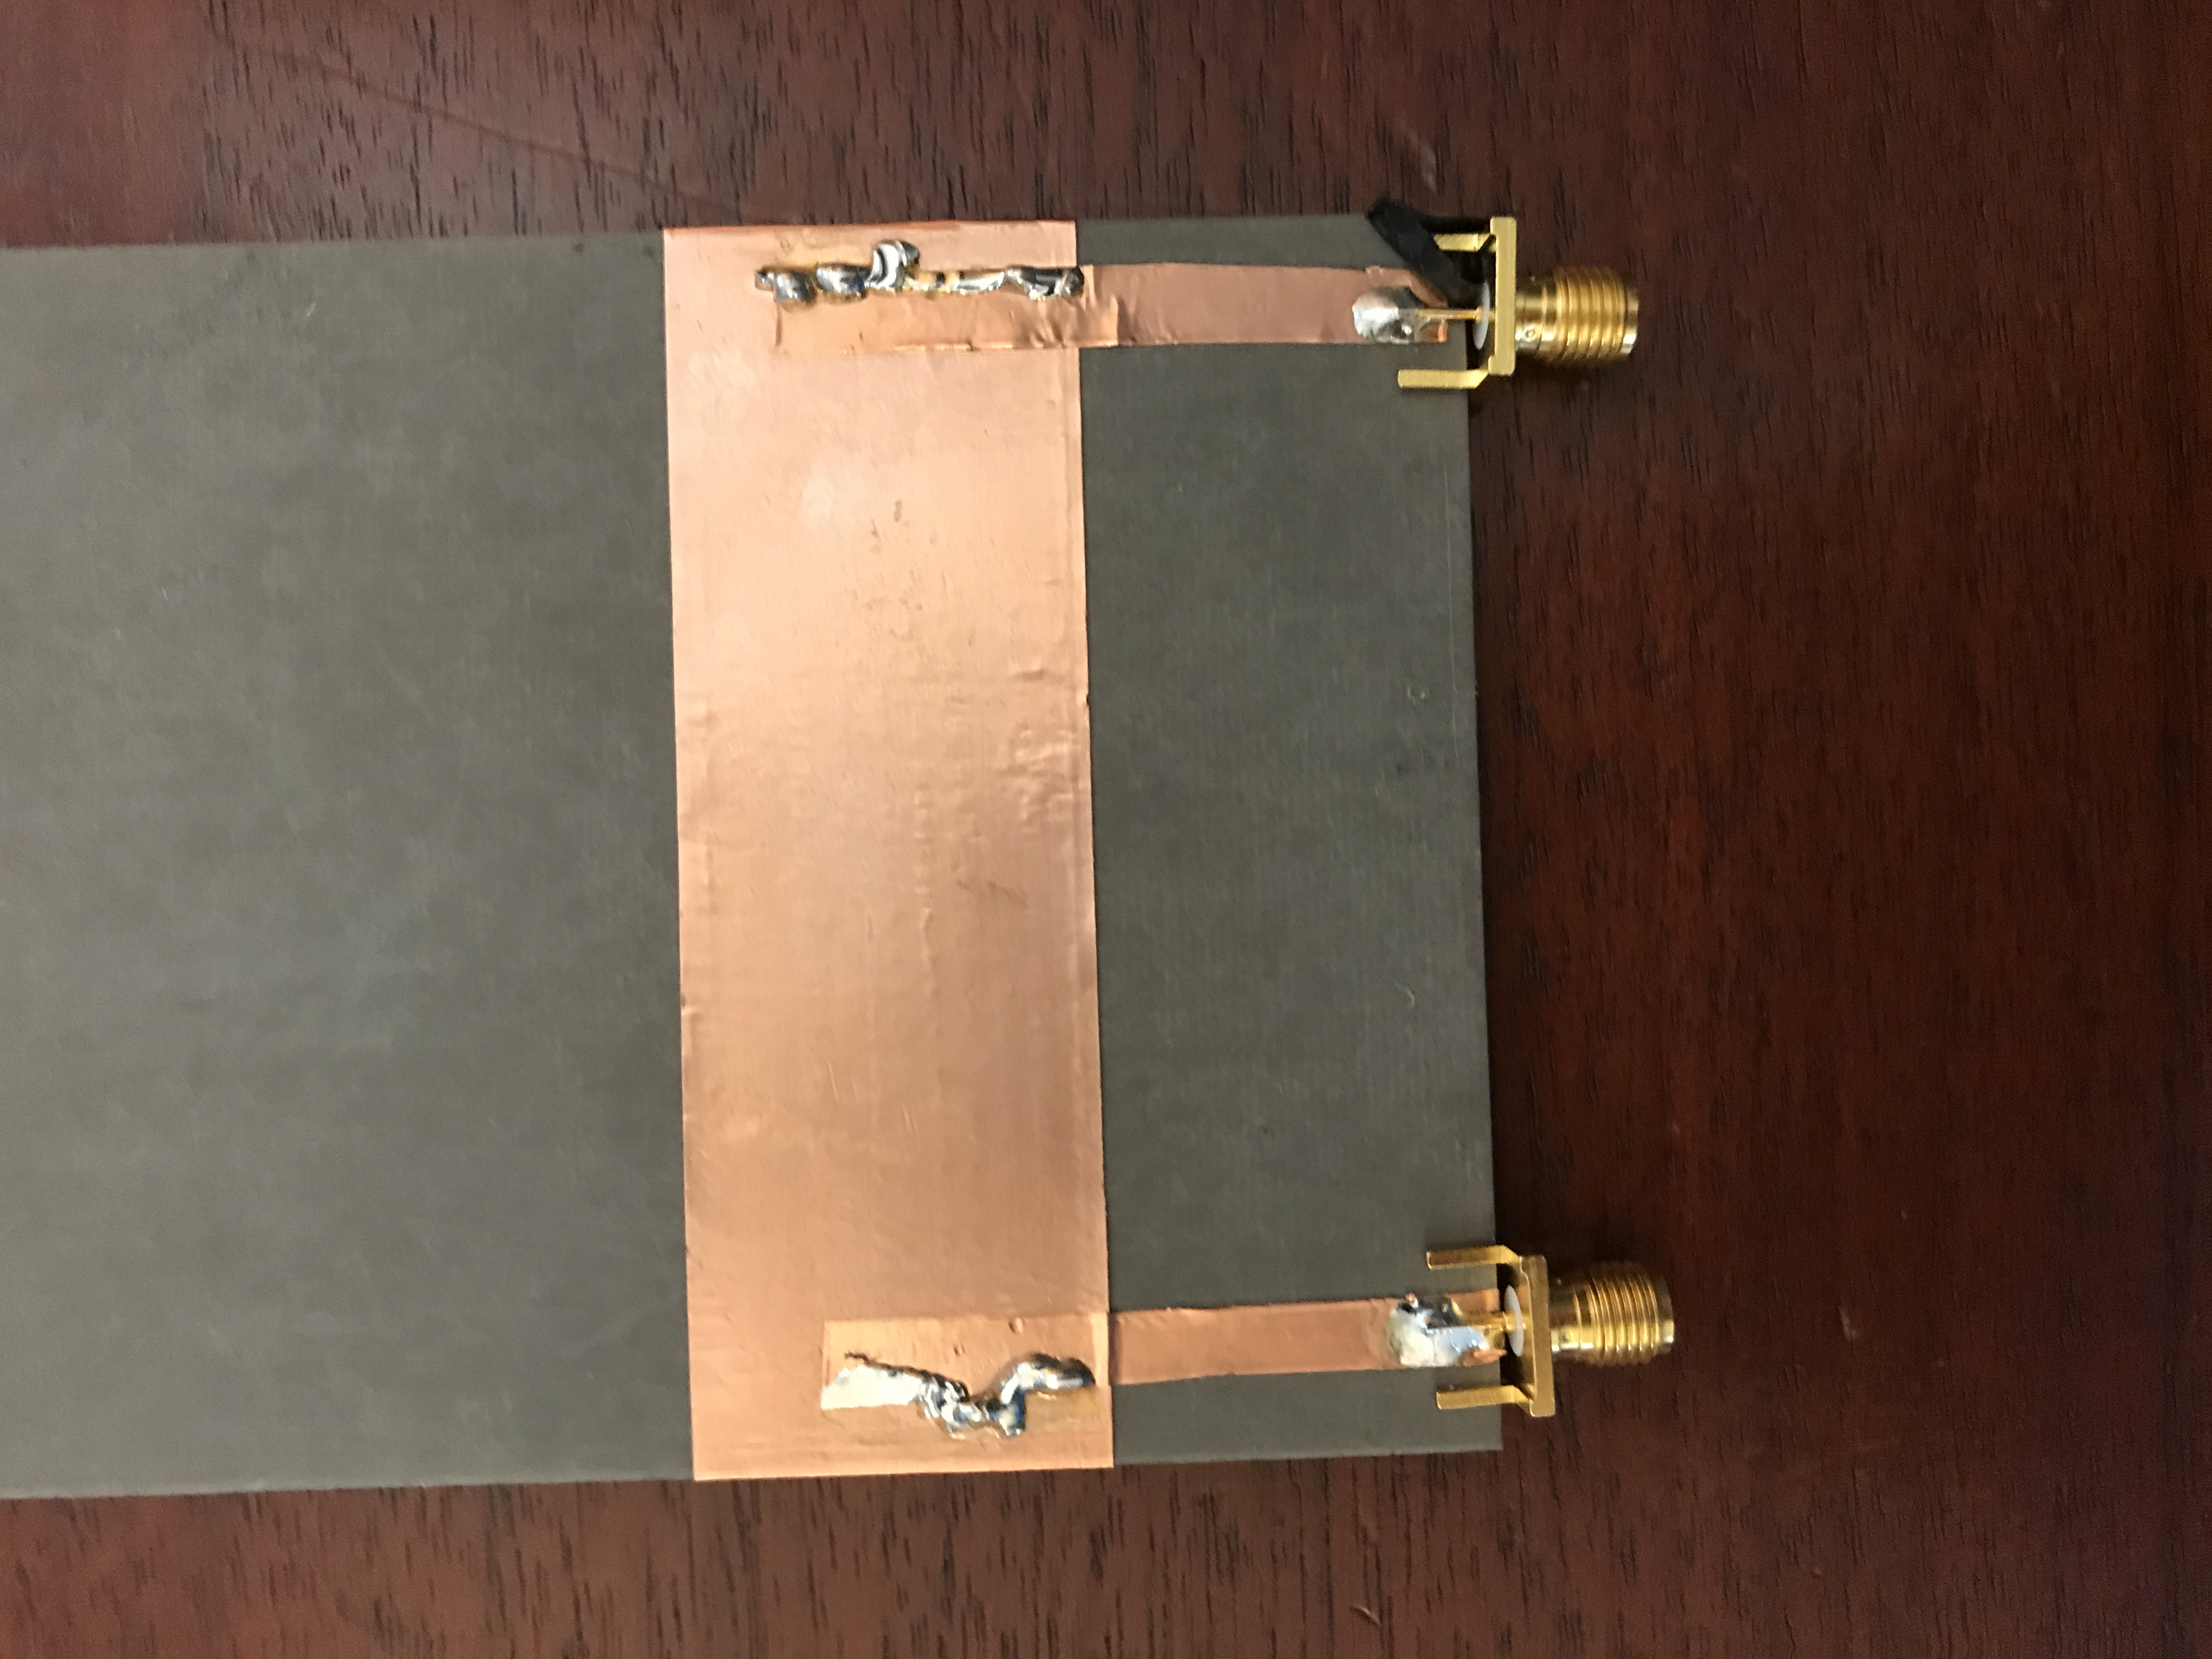
\includegraphics[width=0.8\textwidth, angle = 270]{filter1}
%     \caption{Original width half-wave resonator filter}
% \end{figure}
% \clearpage
\subsection{2.4 GHz half-wave resonator band-pass filter}
In order to build a filter that would work in Wi-Fi range (or at our radar's working frequency), we had to design and build a filter that would only let signal through at around 2.4 GHz. In order to do so, we repeated the above procedure after first calculating the desired length by using: \(D=\frac{m\cdot\lambda_n}{2}\),\(\lambda_n=\frac{\lambda_0}{n}\), \(m=1\),\(\epsilon_r=2.33\), and \(\mu_r=1\). This calulation resulted in a desired length of \(D=0.0409m\). Then we cut the substrate and copper tape appropiately and soldered the connectors. 

% After cutting the substrate boards at the calculated dimensions, we had the following filter:
% \begin{figure}[H]
%     \centering
%     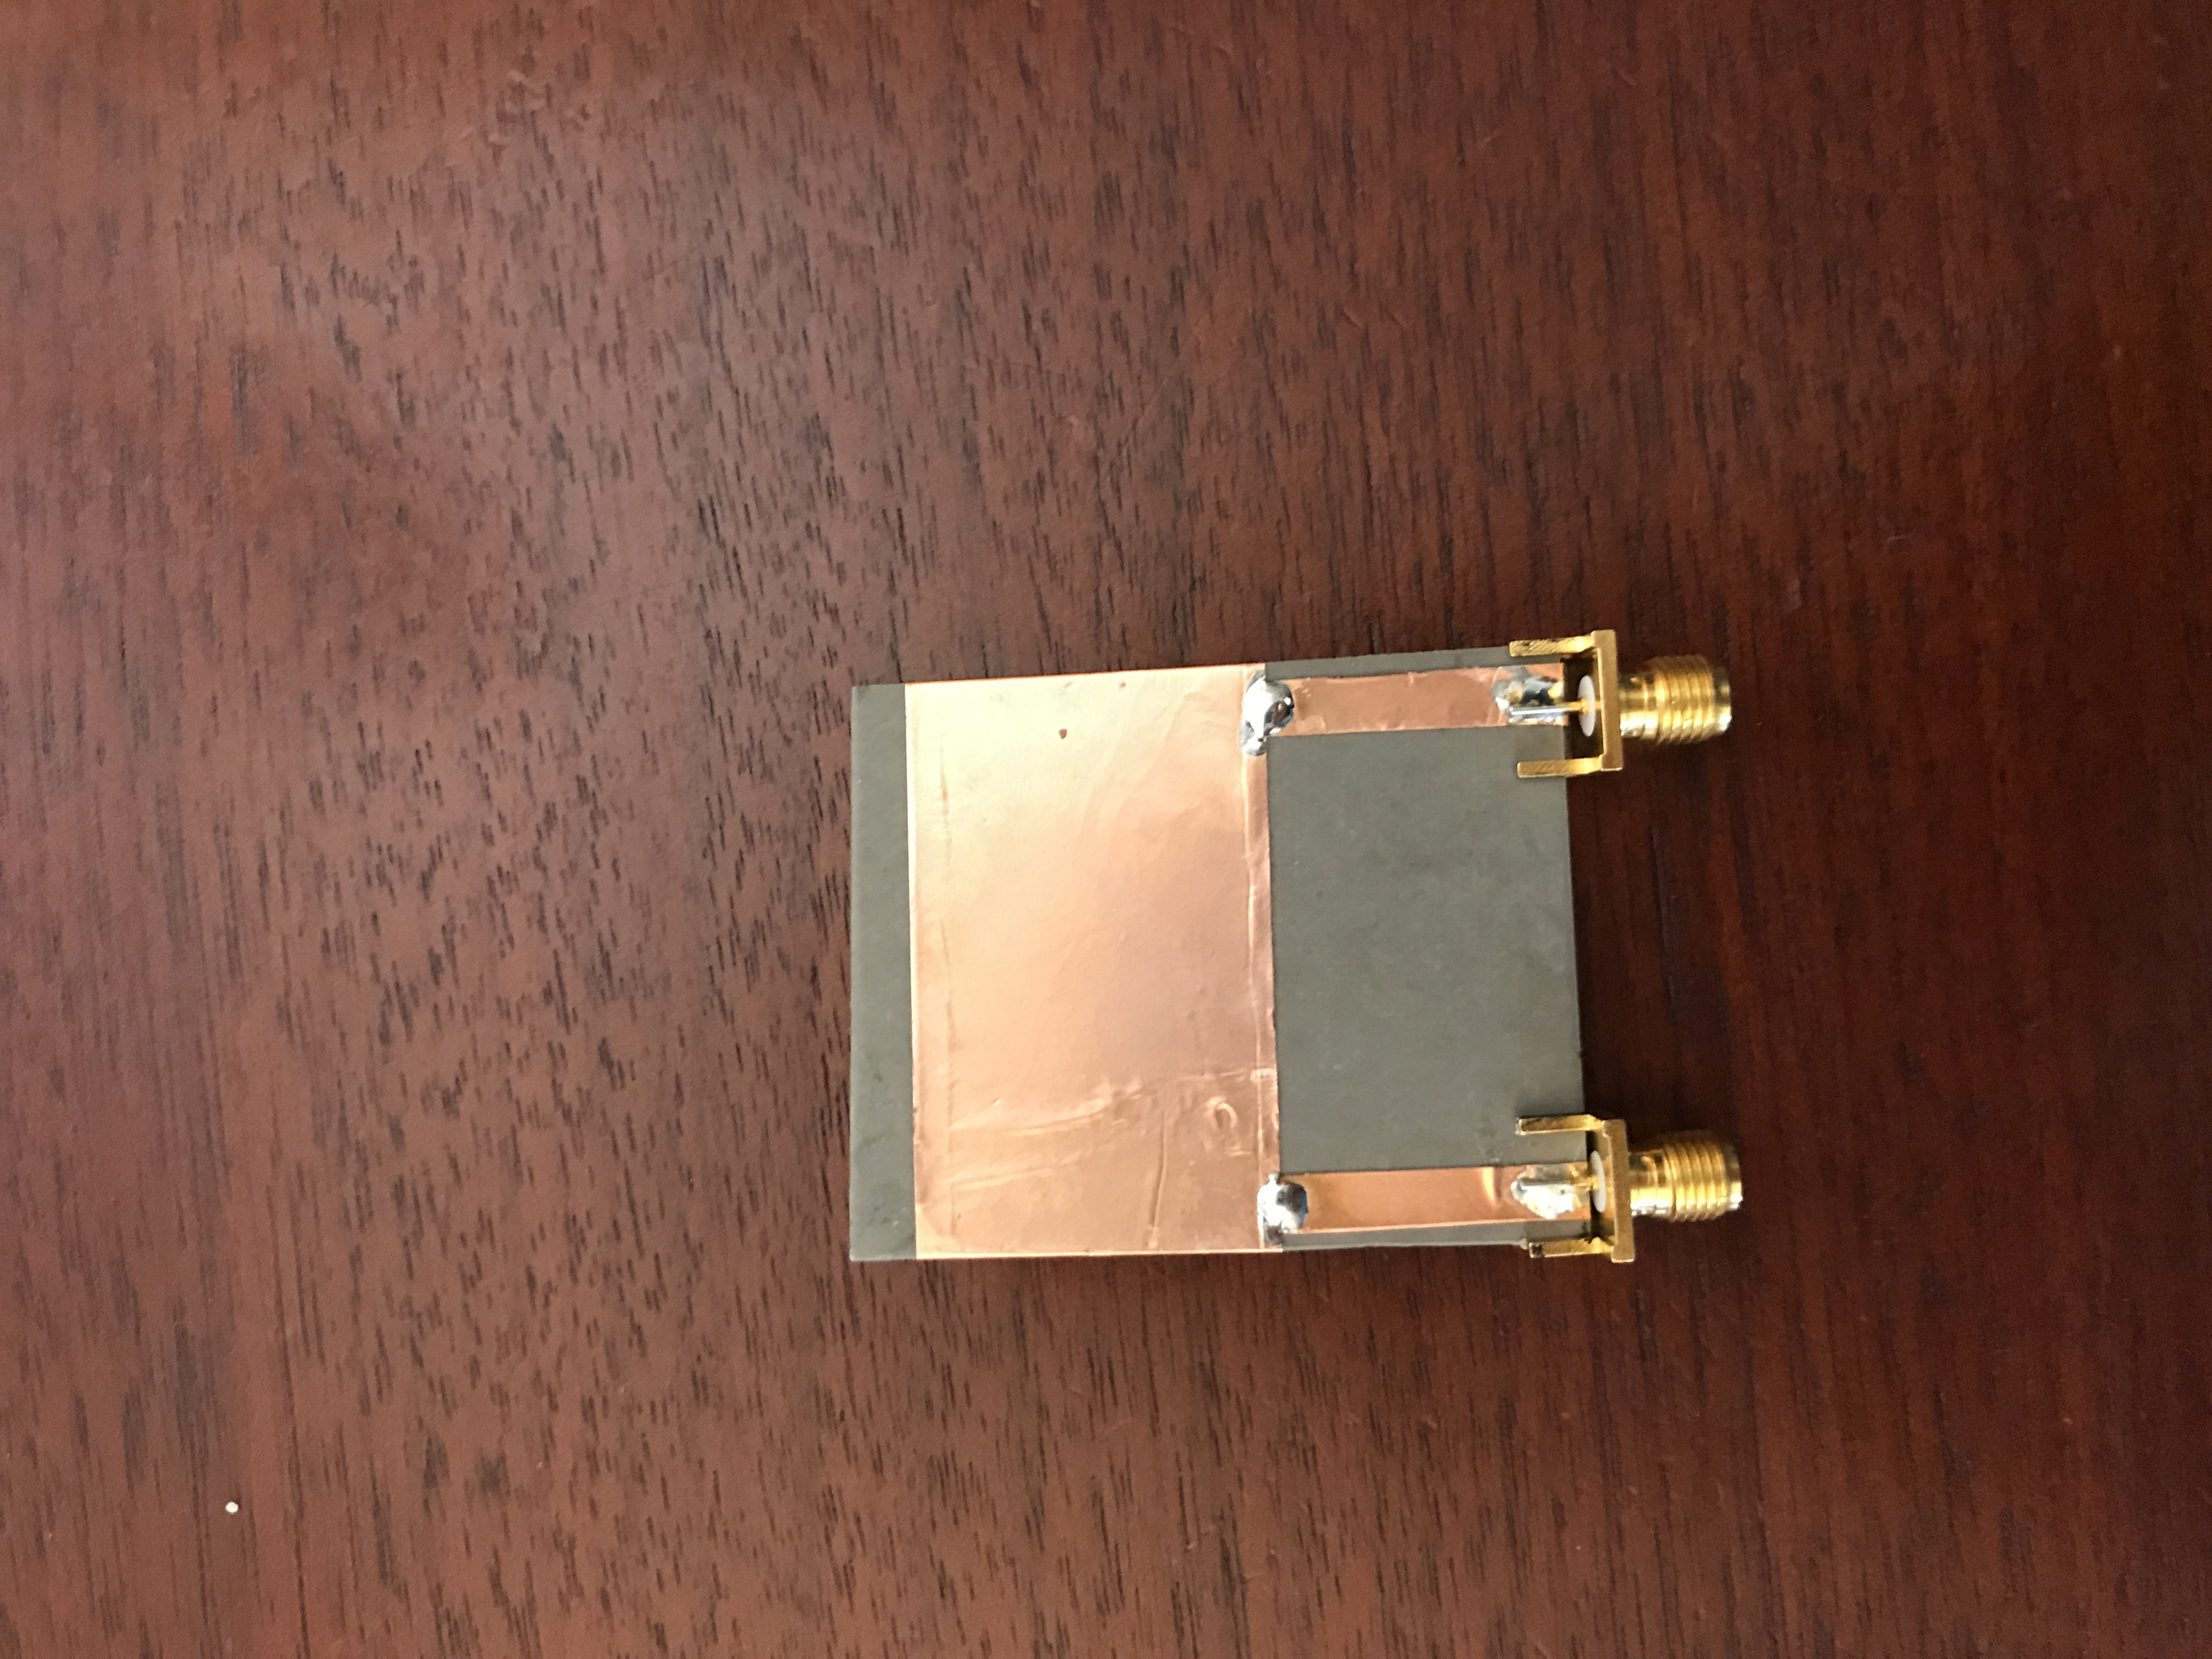
\includegraphics[width=0.8\textwidth, angle = 270]{filter2}
%     \caption{2.4GHz half-wave resonator filter}
% \end{figure}

\subsection{Single stub band-stop filter}
In order to make a band-stop filter, we decided to make a single \(\frac{\lambda}{4}\) stub on a \(50 \Omega\) line. That is designed to transform the open at the end of the stub to a short in parallel with the line which would result in no signal at that frequency. In order to find the correct length, we calculated the wavelength on the substrate, which is \(\lambda=\frac{c/\sqrt{2.33}}{2.4GHz}=0.082m=8.2cm\). That means that our stub has to be \(l=\frac{\lambda}{4}=\frac{8.2}{4}=2.025cm\).
\subsection{Multiple stub band-pass filter}
One other design we developped was a multiple frequency band-stop filter. In order to achieve an approximation of a wide band-pass filter with very sharp edges, we designed a filter that would have multiple band-stop frequencies. 
\section{Results}

\subsection{Half wave resonator Band-Pass filter}
As seen in the yellow line, the short-short band pass filter described first above, returned a relatively promising behavior which is part of the reason we decided to proceed with the same design for the Wi-Fi range. More specifically, the first resonant frequency gave us an attenuation of only around 15 dB at 1.45 GHz. The other resonant frequencies performed even better with attenuations at 8 and 3.5 dB at frequencies of approximately 2.8 and 4.15 GHz respectively.
% \begin{figure}
%     \centering
%     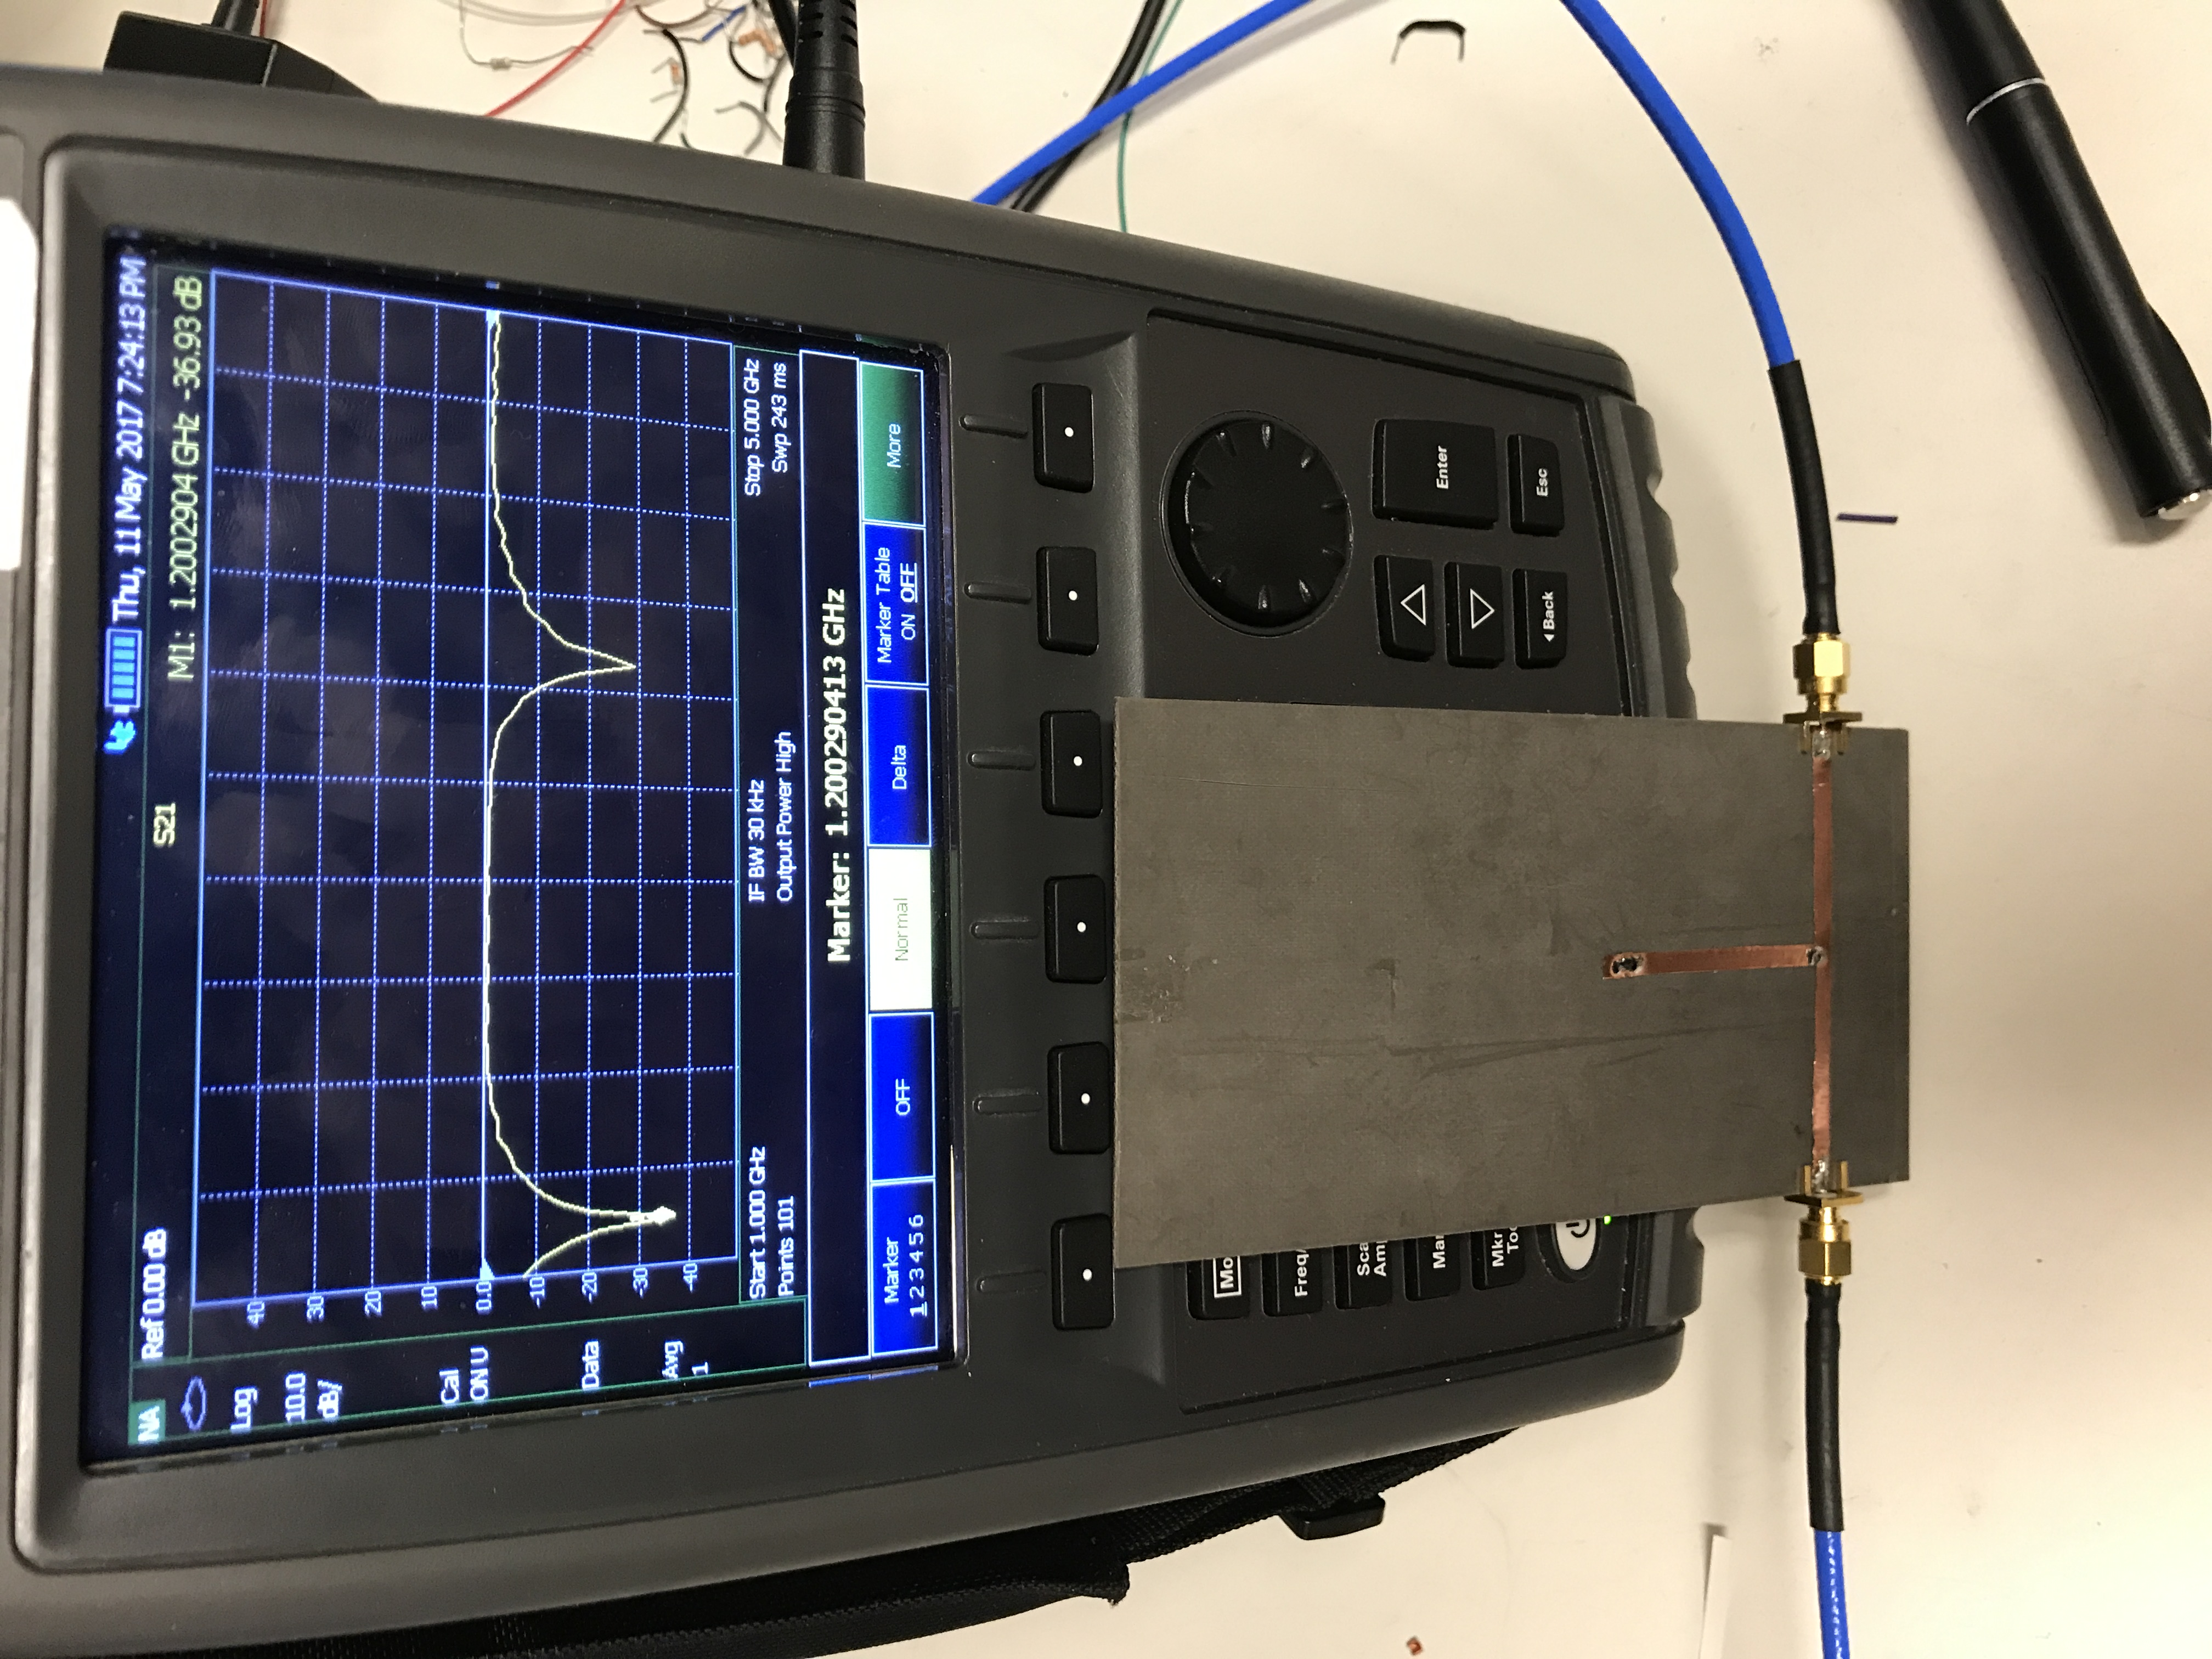
\includegraphics[width=0.8\textwidth, angle=270]{1stub}
%     \caption {single stub measurements}
% \end{figure}
% \subsection{Short-short 2.4 GHz resonator}

\subsection{2.45 GHz half-wave band-pass filter} The 2.45 GHz worked out much
better in the experiments we conducted because of the more careful dimensioning
and manufacturing of the filter. As it can be seen in the figure attached, the
red line representing this filter is attenuated only by 2.6 dB at 2.45 GHz,
while the frequencies immediately outside 2.25-2.75 GHz have more than 20dB
attenuation. This performance was unexpectedly promising for the filter design.  

\subsection{Single stub band-stop filter}
The single-stub quarter wavelenth 2.4 GHz band-stop filter produced again a surprisingly good output. As demonstrated by the blue line on the plot, this filter returned a very sharp "dip" at 2.375 GHz, attenuating the signal by 36dB. The attenuation far from the cut-off frequency was virtually zero. The only problem we faced with this design is in trying to attenuate Wi-Fi signal, as the stub would act as an antenna since we could not properly shield it. This was partially solved by shielding it in aluminum foil (purple line). 

\subsection{Multiple-stub filter}
The multiple band-stop frequency quarter-wavelength stub filter is represented
by the green line on the graph. This filter resulted in a wide passband with
very sharp edges and virtually zero attenuation at around 2.4-2.5 GHz, which was
the respone we were looking for. In addition to that, one can see
low-attenuation peaks at frequencies not attenuated by the stubs or their
resonant frequencies. 

\begin{figure}[H]
    \centering
    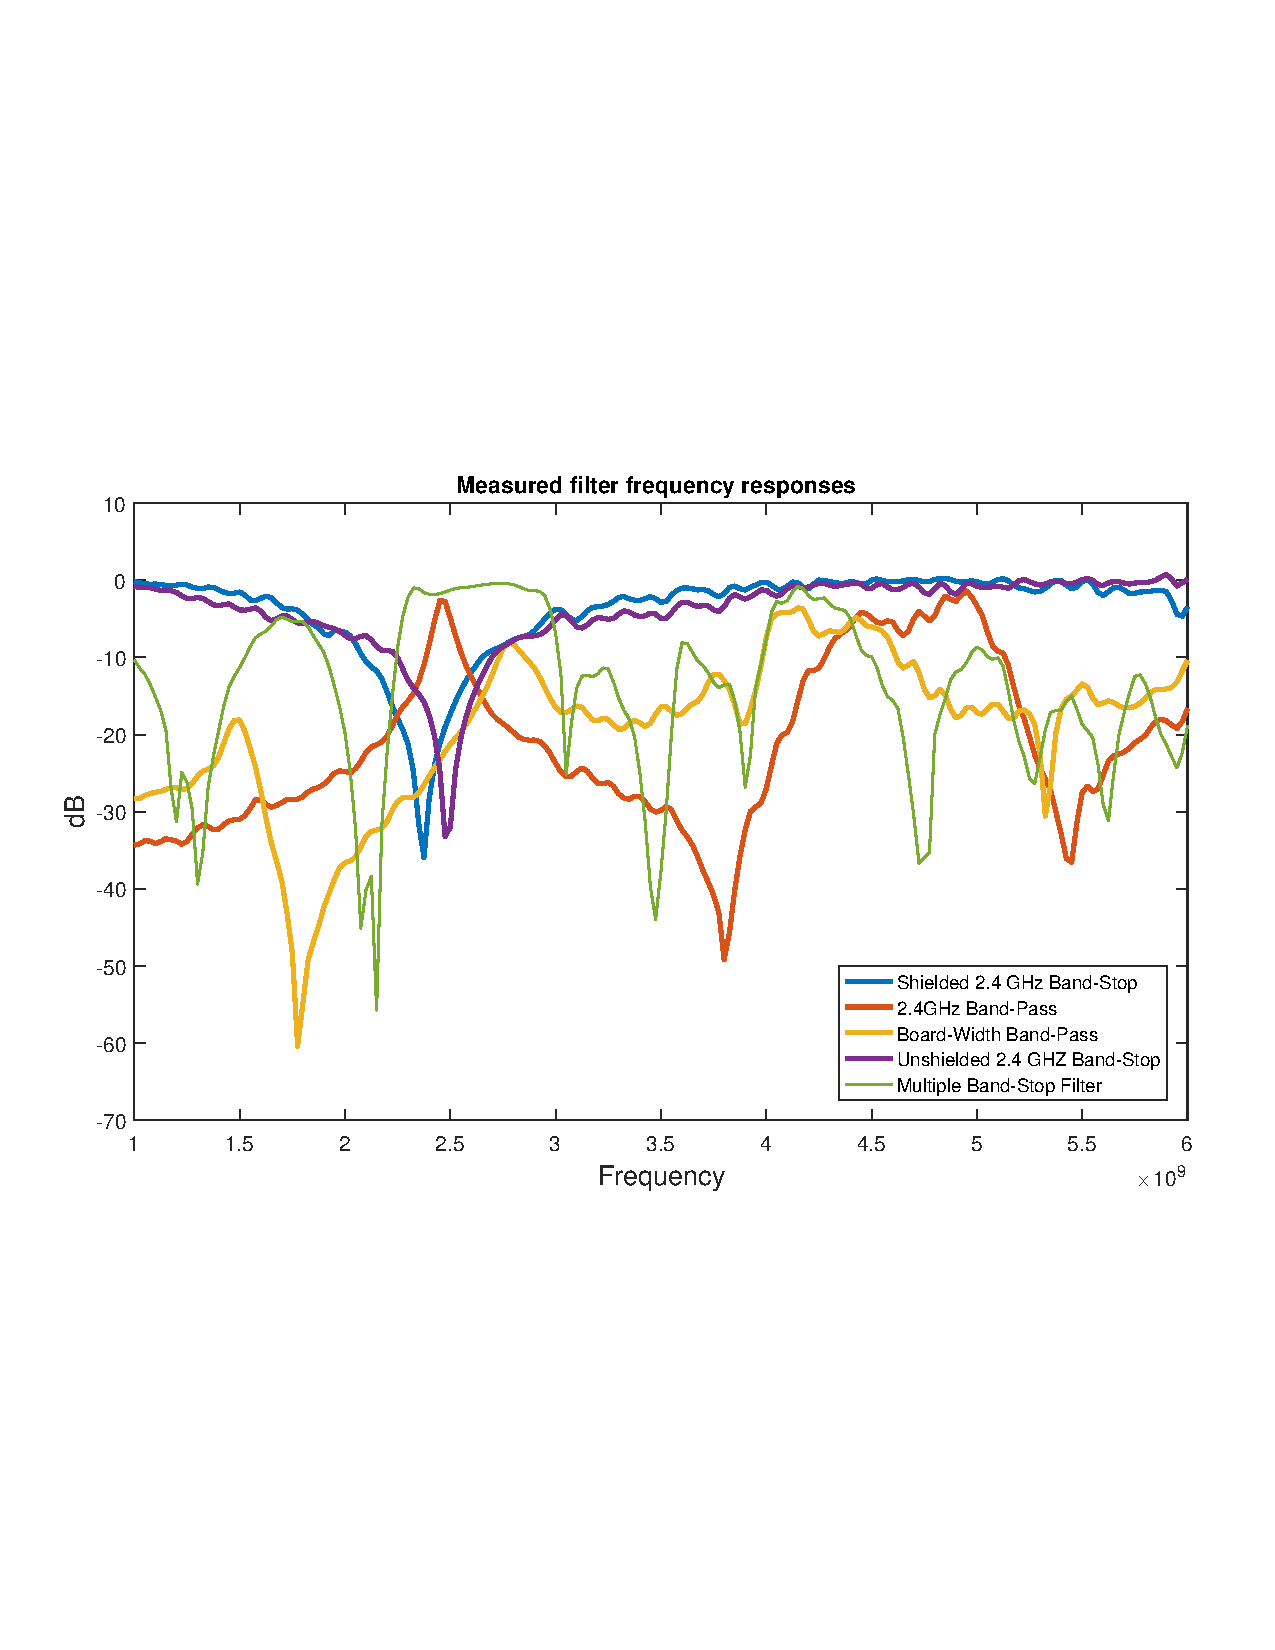
\includegraphics[trim={0.5cm, 7.8cm, 0.2cm, 8cm}, clip=true, width=0.55\textwidth]{graph.pdf}
    \caption{Matlab plot of VNA-measured filter responses}
\end{figure}
\section{Conclusion}
The overall behavior of the filters worked as desired. The band-stop filter was able to attenuate the target signal of 2.45 GHz by 36dB with little sacrifice leaving frequencies below 2GHz and above 3GHz with attenutaion less than 10dB. The designed band-pass filter operated at a bandwidth of 0.07 GHz and at a center frequency of 2.5 GHz. The multiple stub band-stop filter provided wider bandwidth in the passpand region allowing 2.4GHz to pass with nearly 0 dB attenutation. The main limitation with the microstrip design is the cutting of the width of each strip which would affect the characteristic impedance of the line. This factor would create mismatching with impedances with our stubs and main lines therefore causing unwanted reflections at their boundary. It can also be infered that our single stub band-stop filter has a high Voltage Standing Wave Ratio since it produced attenna like effects with being shielded. The proposed filters are all easily implemented without using discrete components and can be integrated into other RF devices and ciruits that target 2.4 GHz.
\end{document}

